%===================================== CHAP 2 =================================

\chapter{Theory}\label{ch:theo}

\section{Introduction to RL Terminology}

\subsection{A Guiding Example}

Many of the concepts in RL are best explained through an example. Consider a version of the 'gridworld' game discussed in p. 76 \cite{barto_sutton_1983} seen in figure \ref{fig:gridworld}. The goal of the game is to move from the starting position in the bottom left to the goal in the top right. The player can move any non-diagonal direction and trying to move off the grid will leave the player in it's previous position.

\begin{figure}[H]
    \centering
    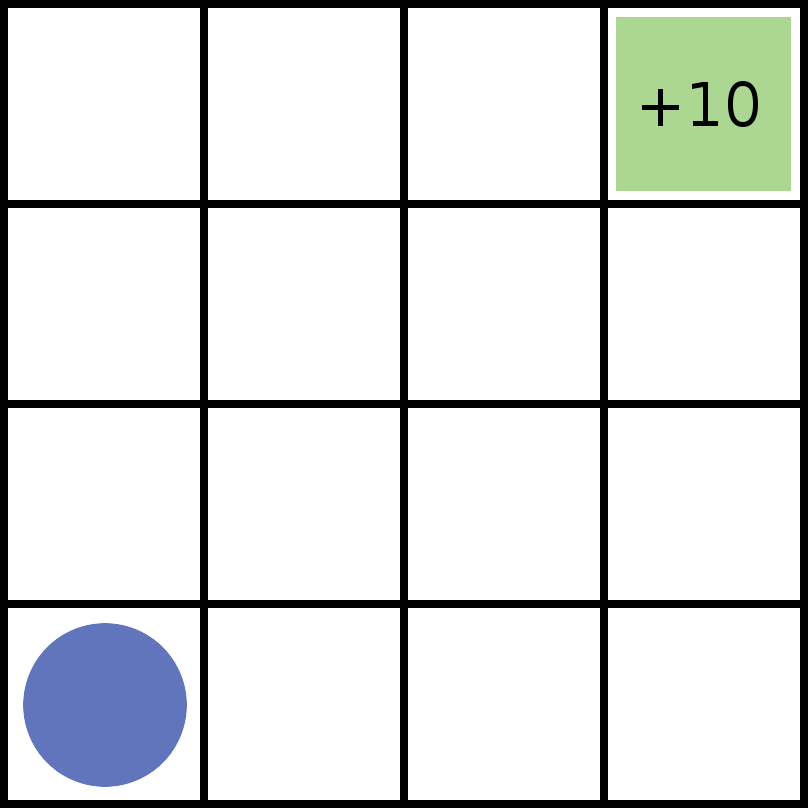
\includegraphics[width=0.5\textwidth, height=1.5in, keepaspectratio]{gridworld.png}
    \captionsetup{width=.5\textwidth}
    \caption{\textbf{Initial State of Gridworld.} The blue circle represents the player, while the green square represents the goal.}
    \label{fig:gridworld}
\end{figure}

In RL literature it is common to decompose this problem into an \textit{agent} and \textit{environment}. The agent is the object which can perform actions. In the gridworld example this is the player. The environment is what the agent interacts with and what returns information about the game. 

In general the environment consists of two things. First is the state, which defines what is going on in the environment. In the gridworld example this could be the players position on the grid. Second is the reward, some signal that what the agent is doing is right or wrong. This could be -1 for every action taken and +10 for reaching the goal. Note that one does not always need a reward per action. For example in chess the reward can be purely +1 for a win, -1 for a loss and 0 for everything else. This agent environment decomposition is visualized in figure \ref{fig:agent-env}.

\begin{figure}[H]
    \centering
    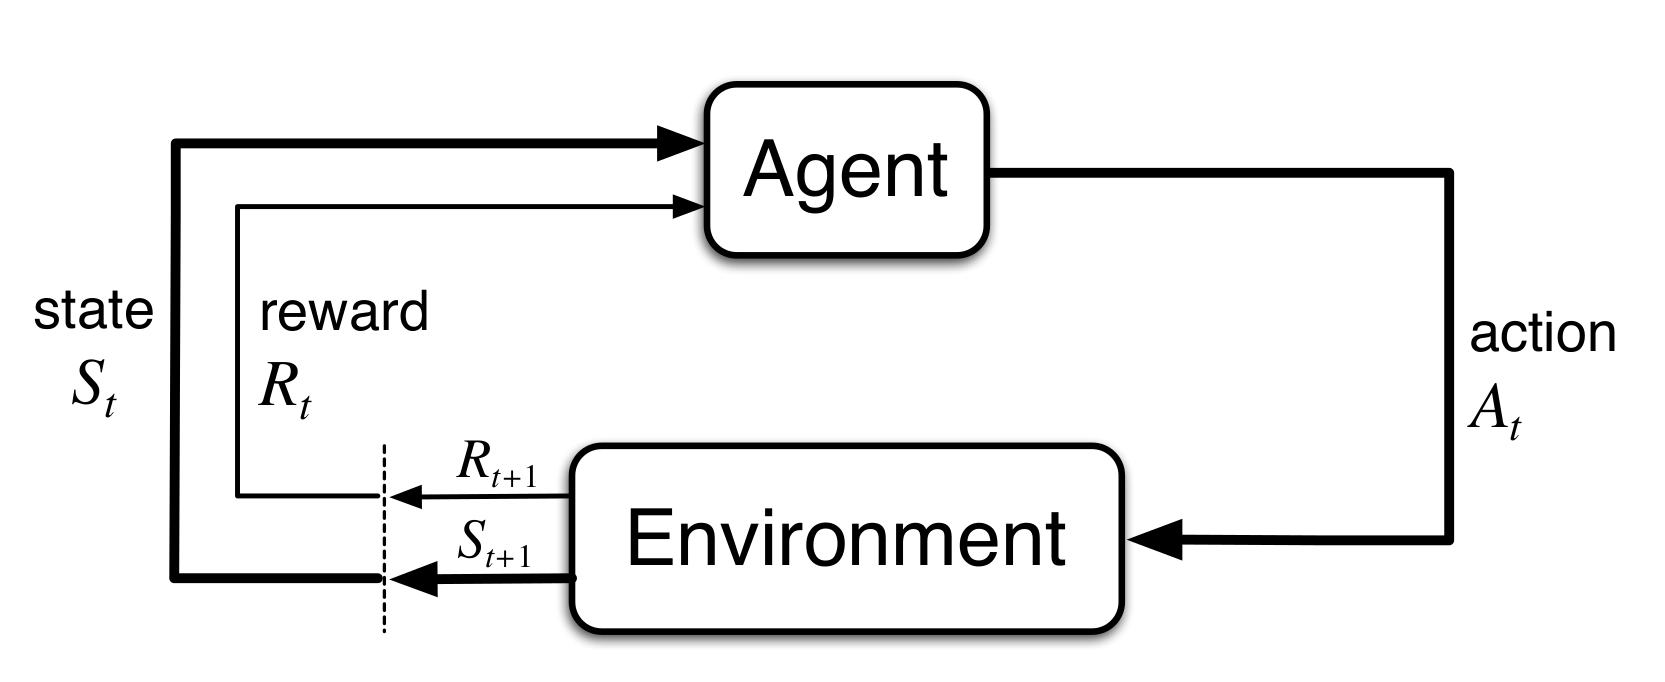
\includegraphics[width=0.5\textwidth]{agent-env.png}
    \captionsetup{width=.5\textwidth}
    \caption{\textbf{Visualization of the Agent and Environment.} The figure is from \citep[p.~48]{sutton_barto_2018}}
    \label{fig:agent-env}

\end{figure}


Upon reaching the goal the game is over, making the goal state a \textit{terminal state}. Environments with terminal states are called \textit{episodic} as during training the game must be reset to keep playing. If instead the player is teleported back to the start and can keep playing it is a \textit{continuous} environment.

\subsection{Tabular Markov Decision Process}

Though the applications of RL are broad, most of the theory behind RL has been developed around simpler problems that have the two following attributes. Firstly the problem should be tabular, meaning that the number of combinations of states and actions should be small enough to fit in memory. Secondly the problem should follow a Markov Decision Process (MDP). \cite[p.~23]{barto_sutton_1983}\citep[p.~57]{powell_2011} 

MDPs build on the concept of Markov chains (MC). According to \cite{ross_2014} a MC is a stochastic process consisting of a sequence of successive random variables $S_t$ that can take values from a countable set $\mathbb{S}$. These are called states. The state at a time step is denoted $S_t$ for $t \in T$ where $T$ is a discrete or continuous set that often relates to the time step for the occurrence. For example, in gridworld $S_2$ would represent the players position after two actions.

In a MC the next state is dependent only on the current state. This is known as the Markov Property. Thus a transition matrix is defined consisting of probabilities

\begin{equation}
    p_{s,s'} = P(S_t=s'|S_{t-1}=s) \quad \text{for} ~ s',s \in \mathbb{S}
\end{equation}

which denote the probability of transitioning from state $s$ to state $s'$.

In a MDP two additional factors are added, an action $A$ from a discrete action set $\mathbb{A}$ and a reward $R$ from a real set $\mathbb{R}$. The transition probability is now defined as

\begin{align}
    P(s',r|s,a) = P(S_{t}=s', R=r|S_{t-1}=s, A=a)
\end{align}

Essentially a MDP allows for an action to be taken at each state which in turn effects the probability distribution of the next state. In addition the transition to a new state returns a numerical reward $R$. \citep[p.~38]{sutton_barto_2018}. 

From this definition one can model the gridworld example as a MDP. Given a player state, an action can be chosen to move to North, East, West or South. As long as the action leads to a state that is on the grid, the transition probability is one to the desired square and zero for all other squares. If the action leads off-grid the transition probability is one to stay in the same square. This follows the Markov property as the transition probability is only dependent on the current state and action. Finally, performing an action the agent receives a reward of +10 if it reaches the goal and -1 otherwise.  

\section{Dynamic Programming solutions to Tabular MDPs}

\subsection{Bellman Equation}

Given a MDP the goal in RL is to maximize the total reward returned. The total discounted reward can be defined as

\begin{equation}
    \label{eq:return}
    G_t(s) = \sum_{k=0}^\infty \gamma^kR_{t+k+1}(A_t| S_t=s)\quad \text{where} ~ 0 << \gamma < 1.
\end{equation}

The future rewards are discounted by a factor of $\gamma$ to ensure the convergence of the methods that follow when used on endless environments. Episodic environments can have $\gamma=1$, however in practice it is still common to use $\gamma < 1$ as it is the equivalent of weighting short-term rewards more than the possibly less reliable long-term rewards.

The total reward is influenced by the actions taken in the MDP so the aim is to estimate a function that takes in the current state and outputs the probability of performing an action. This is refereed to as the policy and is denoted

\begin{equation}
    \pi = P(A=a|S_t=s).
\end{equation}

The notation in equation \ref{eq:return} is often shortened for the sake of readability. For the rest of this project $G_t(s)$ will be denoted as $G_t$ and $R_t(A_t|S_t=s)$ is denoted $R_t$. The optimization of the process can then be defined as 

\begin{equation}
    \max_\pi ~ \mathbb{E_\pi}\big[G_t]
    \label{eq:cost_function}
\end{equation}

where $G_t$ is the total discounted reward when following policy $\pi$.

To solve this maximization problem one must be able to calculate $\mathbb{E_\pi}\big[G_t]$ given a policy $\pi$. Consider equation \ref{eq:cost_function} from a given state. 

\begin{equation}
    v_\pi(s_t) = \mathbb{E}_\pi[G_t|S_t=s_t]
    \label{eq:value_function}
\end{equation}

Equation \ref{eq:value_function} is known as the \textit{value function}. It is the expected reward to be gained from the state $s_t$ and onward while following policy $\pi$. In other words this represents how good it is to be in state $s_t$ when following policy $\pi$. Expanding $G_t$ gives

\begin{equation}
    v_\pi(s_t)  = \mathbb{E}_\pi[R_{t+1} + \gamma G_{t+1}|S_{t+1}=s_{t+1}].
    \label{eq:expanded_value_function}
\end{equation}

Noting that 

\begin{equation}
    \mathbb{E}_\pi[R_t] = \mathbb{E}[R_t|A_t=a] = \mathbb{E}[r_t] = r_t
\end{equation}

one can rewrite equation \ref{eq:expanded_value_function} as 

\begin{align}
\begin{split}
    &=  r_{t+1} + \gamma\mathbb{E}_\pi[G_{t+1}|S_{t+1}=s_{t+1}] \\
    &= r_{t+1} + \gamma v_\pi(s_{t+1}).
    \label{eq:bellman_value_function}
\end{split}
\end{align}

There is one such formula per state, so the whole environment is represented by a system of $|\mathbb{S}|$ simultaneous linear equations with $|\mathbb{S}|$ unknown values $v_\pi(s)$. This decomposition was first suggested by Richard Bellman\citep{bellman_1957} and hence is called the Bellman Equation. The process of solving the above is known as \textit{policy evaluation} in RL literature.

The value function decomposition can also be expanded to the action-value function which represents how 'good' each action $a$ from state $s$ is.

\begin{align}
\begin{split}
    \label{eq:act_value_function} 
    Q(s_t, a) &=  \mathbb{E}_\pi[G_t|S_t=s_t, A_t=a] \\
    Q(s_t, a) &= \mathbb{E}\big[R_{t+1}(S_t, A_t) + \gamma v(S_{t+1})|S_t=s_t, A_t = a\big]
\end{split}
\end{align}

In certain situations, which will be discussed at a later stage, equation \ref{eq:act_value_function} can be a more useful decomposition.

To conclude, a naive way to solve equation \ref{eq:cost_function} is then to calculate the value or action-value function for all policies and simply pick the policy that has the highest value for the initial state. This solution is guaranteed optimal but computationally inefficient and in practice unfeasible for many environments.

\citep[p.~58-61]{powell_2011}\citep[p.~59]{sutton_barto_2018}

\subsection{Value and Policy Iteration}

If one can perfectly model the environment and the MDP has a finite number of states the Bellman Equation can be solved using dynamic programming. This means one has access to all the transition probabilities for all possible state-action pairs. The following overview of the dynamic programming method is summarized from \cite[p.~74-84]{sutton_barto_2018}.

\subsubsection{Policy Evaluation}

The calculation of the value function of a given policy is known as policy evaluation. As an alternative to calculating the value function from the system of $|S|$ equations there is the iterative method

\begin{equation}
    v_\pi^{(k+1)}(s) = \mathbb{E}[R_{t+1} + \gamma v_\pi^{(k)}(S_{t+1})| S_t=s]
    \label{eq:policy_eval}
\end{equation}

and terminating the iteration when 

\begin{equation}
    \| v^{k+1} - v^k \| < \epsilon \quad for \quad \epsilon > 0.
    \label{eq:policy_eval_termination_condition}
\end{equation}

This converges to the value function given that $v_\pi(S)$ exists, which is true when $\gamma < 1$ or that an episode is guaranteed finite.

%Add pseudocode to appendix

\subsubsection{Policy Iteration}

This policy evaluation method can then be used to create a new policy $\pi'$ by greedily picking actions in each state $S_t$ based on newly calculated $v_\pi(S_{t+1})$. 

\begin{equation}
    \pi'(s) = \argmax_{a\in \mathbb{A}_t} \mathbb{E}\big[R_{t+1} + \gamma v_\pi(S_{t+1})|S_t=s, A_t=a\big]
    \label{eq:policy_iter}
\end{equation}

This process is called policy improvement. It can be proven that the new policy $\pi'$ fulfills $v_{\pi'}(s) \geq v_\pi(s) ~~ \forall s \in \mathbb{S}$ meaning $\pi'$ is as good or better than the policy $\pi$ used for policy evaluation. \citep[p.~78-79]{sutton_barto_2018}

Repeatedly running the policy evaluation and improvement steps above results in a monotonically improving policy and value function. For a finite MDP this will result in finding the policy that maximizes the discounted total reward.

%Add pseudocode to appendix

\subsubsection{Value Iteration}

Policy iteration as described above requires that equation \ref{eq:policy_eval} converges before improving the policy. The basis for value iteration is that the policy evaluation does not need to converge first. Instead it combines both steps into one simple update rule:

\begin{equation}
    v_{k+1}(s) = \max_{a \in \mathbb{A}_t} \mathbb{E}\big[R_{t+1} + \gamma v_{k}(S_{t+1})|S_t = s, A_t = a)\big].
    \label{eq:value_iter}
\end{equation}

The termination condition is given by equation \ref{eq:policy_eval_termination_condition} as in policy iteration. When the value function has converge a policy is given by

\begin{equation}
    \pi(s) = \argmax_{a\in \mathbb{A}_t} \mathbb{E}\big[R_{t+1} + \gamma v(S_{t+1})|S_t=s, A_t=a\big]
\end{equation}

The result of running value iteration on the gridworld example can be seen in figure \ref{fig:value_it}

\begin{figure}[H]
\centering
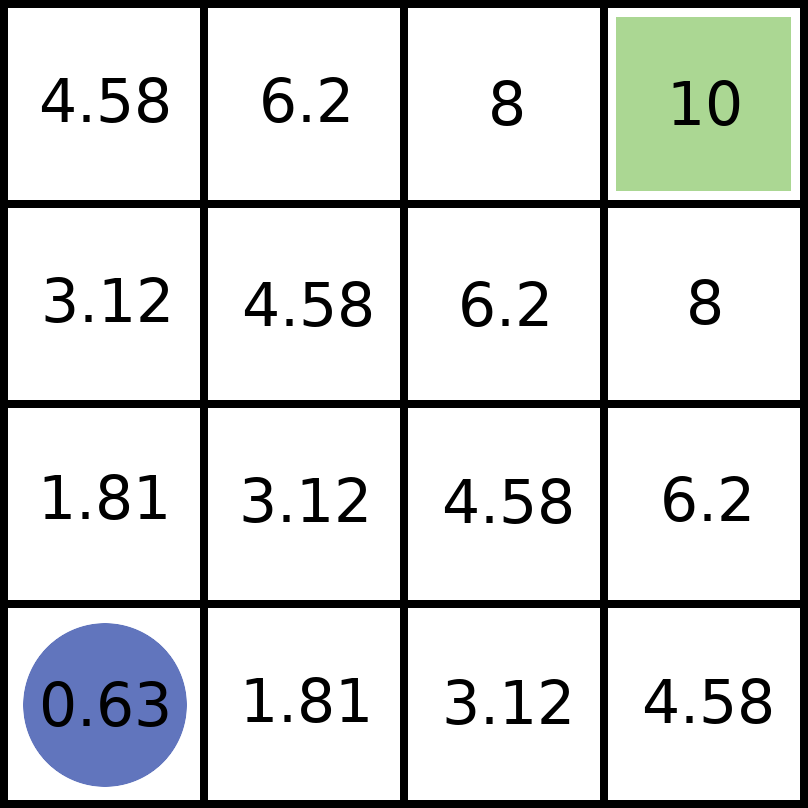
\includegraphics[width=0.5\textwidth, height=1.5in, keepaspectratio]{gridworld_value.png}
\captionsetup{width=.7\linewidth}
\caption{\textbf{Value Iteration run on gridworld example}. A discount rate of $0.9$ was used. Note that the closer the player is to the green zone, the higher the point sum.}
\label{fig:value_it}
\end{figure}

As in policy iteration it can be proved that value iteration converges to the optimal value and policy function given a finite MDP. \citep[p.~89-93]{powell_2011}.

\subsection{Limitations of Value and Policy iteration}

There are many situations where value and policy iteration(equation \ref{eq:policy_iter} and \ref{eq:value_iter}) cannot be used to solve MDPs. \cite{powell_2011} (p.~5-6) discusses the curse of dimensionality. When there are too many states or actions it is computationally infeasible to run the above algorithms. \cite{sutton_barto_2018} (p.~91, 119) points out that a suitable environment model isn't always available, which makes it impossible to directly calculate $V(S_{t+1})$.

\section{Reinforcement Learning solutions to Tabular MDPs}

RL builds on a different approach than the methods discussed above. Consider the gridworld example. In value and policy iteration the game is never played during training. The entire policy is learned based on a model of how the game works. In a RL approach the agent is given access to an environment and tries to learn the optimal policy based on experiences from interacting with the environment.

\subsection{Advantages of Learning From Experience}

The experiences used to train the agent are often referred to as \textit{samples} in RL literature as they can be viewed as samples from the underlying MDP. These samples are simply a set of states, actions and rewards that resulted from interacting with the environment. The specific size of a sample varies based on the method and can be anything from one state transition to all the transitions within an episode. 

However this thesis also contains discussion about random samples and sampling from statistical models of value functions. To avoid confusion between these two concepts samples from the environment will be referred to as \textit{experiences} throughout this thesis. 

There are two main reasons why learning from experiences can be useful. In many cases one can generate experiences from the environment without having a model of all the dynamics of the system. Consider for example trying to maximize profit by buying and selling a stock. There are far too many factors and unknowns to be able to perfectly predict the future price of a stock. However for the correct stock there can exist decades of pricing history. This history can be used as experiences to train a RL model. This is a common problem, where creating an accurate model of the environment can be a lot more challenging then drawing experiences from the environment.

Secondly reinforcement learning algorithms can focus on modeling promising states and neglect states that clearly lead to sub-optimal results. In contrast the dynamic programming methods run the same number of calculation for all states. This allows reinforcement learning to solve larger MDPs than DP methods. \citep[p.~115]{sutton_barto_2018}

\subsection{Temporal Difference learning}

\subsubsection{Generalized Policy Iteration}

\begin{wrapfigure}[12]{r}{0.3\textwidth} %this figure will be at the right
    \vspace*{-1cm}
    \centering
    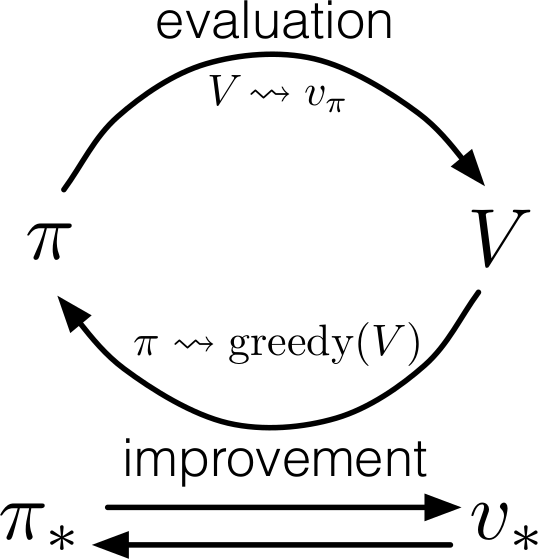
\includegraphics[width=0.3\textwidth]{GPI}
    \caption{\textbf{Visualization of GPI.} Taken from p. 86 \cite{sutton_barto_2018}}
    \label{fig:GPI}
\end{wrapfigure}

There are two major paradigms in reinforcement learning: generalized policy iteration (GPI) and policy gradient (PG) methods. The focus of this project will be on generalized policy iteration. These are methods that follow the same structure as value and policy iteration. Essentially a GPI methods are characterized by the fact that they try to model the value function of the MDP. This value function is then used to improve the policy. The improved policy then leads to a new value function, and the cycle repeats. A visualization of this can be seen in figure \ref{fig:GPI} \citep[p.~86]{sutton_barto_2018}.

\subsubsection{Learning from experience}

How to learn a value function from experiences is not obvious. Consider the case of trying to learn to play chess. One way to model this game as a MDP is to give a reward upon winning the game. Given one game, how does one propagate the final reward to the states that lead up to the result?

One set of methods are Monte Carlo methods. These simply update the values of the states that were visited before the reward. Mathematically 

\begin{equation}
    V_\pi(S_t) = V_\pi(S_t) + \alpha \big[G_t - V_\pi(S_t)]
\end{equation}

where $\alpha$ is the step size of the update. This can be viewed as using $G_t$ as the target value that is trying to be modeled. Note that using this method one must wait until the end of the game before updating values.

Temporal difference methods instead update the value function every time a step is taken in the MDP. To do one can replace $G_t$ by the one step return $G_{t:t+1} = R_{t+1} + \gamma V_{t+1}(S_{t+1})$ giving

\begin{equation}
    V_\pi(S_t) = V_\pi(S_t) + \alpha \big[R_{t+1} + \gamma V_\pi(S_{t+1}) - V(S_t)\big].
    \label{eq:one-step}
\end{equation}

In this case the target is based on the estimated value of the next state and the reward gained in the step taken. In reinforcement learning literature this is referred to as bootstrapping the target value.

Since equation \ref{eq:one-step} considers the reward after one step it is called the 1-step TD method. However one doesn't have to chose between the monte carlo return or the one-step bootstrap. $G_t$ can be replaced by any $n$-step return. For example a 3-step TD method

\begin{equation}
    V_\pi(S_t) = V_\pi(S_t) + \alpha \big[R_{t+1} + \gamma R_{t+2} + \gamma^2 R_{t+3} + \gamma^3V_\pi(S_{t+3}) - V(S_t)\big].
\end{equation}

As $n\rightarrow\infty$ the $n$-step update becomes a Monte Carlo update. The choice of $n$ can be seen as a bias-variance trade-off. The variance in a target in RL comes from a combination of stochastic transitions in the environment and different or stochastic policies. The total return based on the Monte Carlo target has variance from both these sources over all steps in an episode. A 1-step episode only has variance from the single transition and action choice but uses a biased bootstraped target value. The minimal error will then be somewhere between the two as can be seen in in figure \ref{fig:bias-variance}.

\begin{figure}[H] %this figure will be at the right
    \centering
    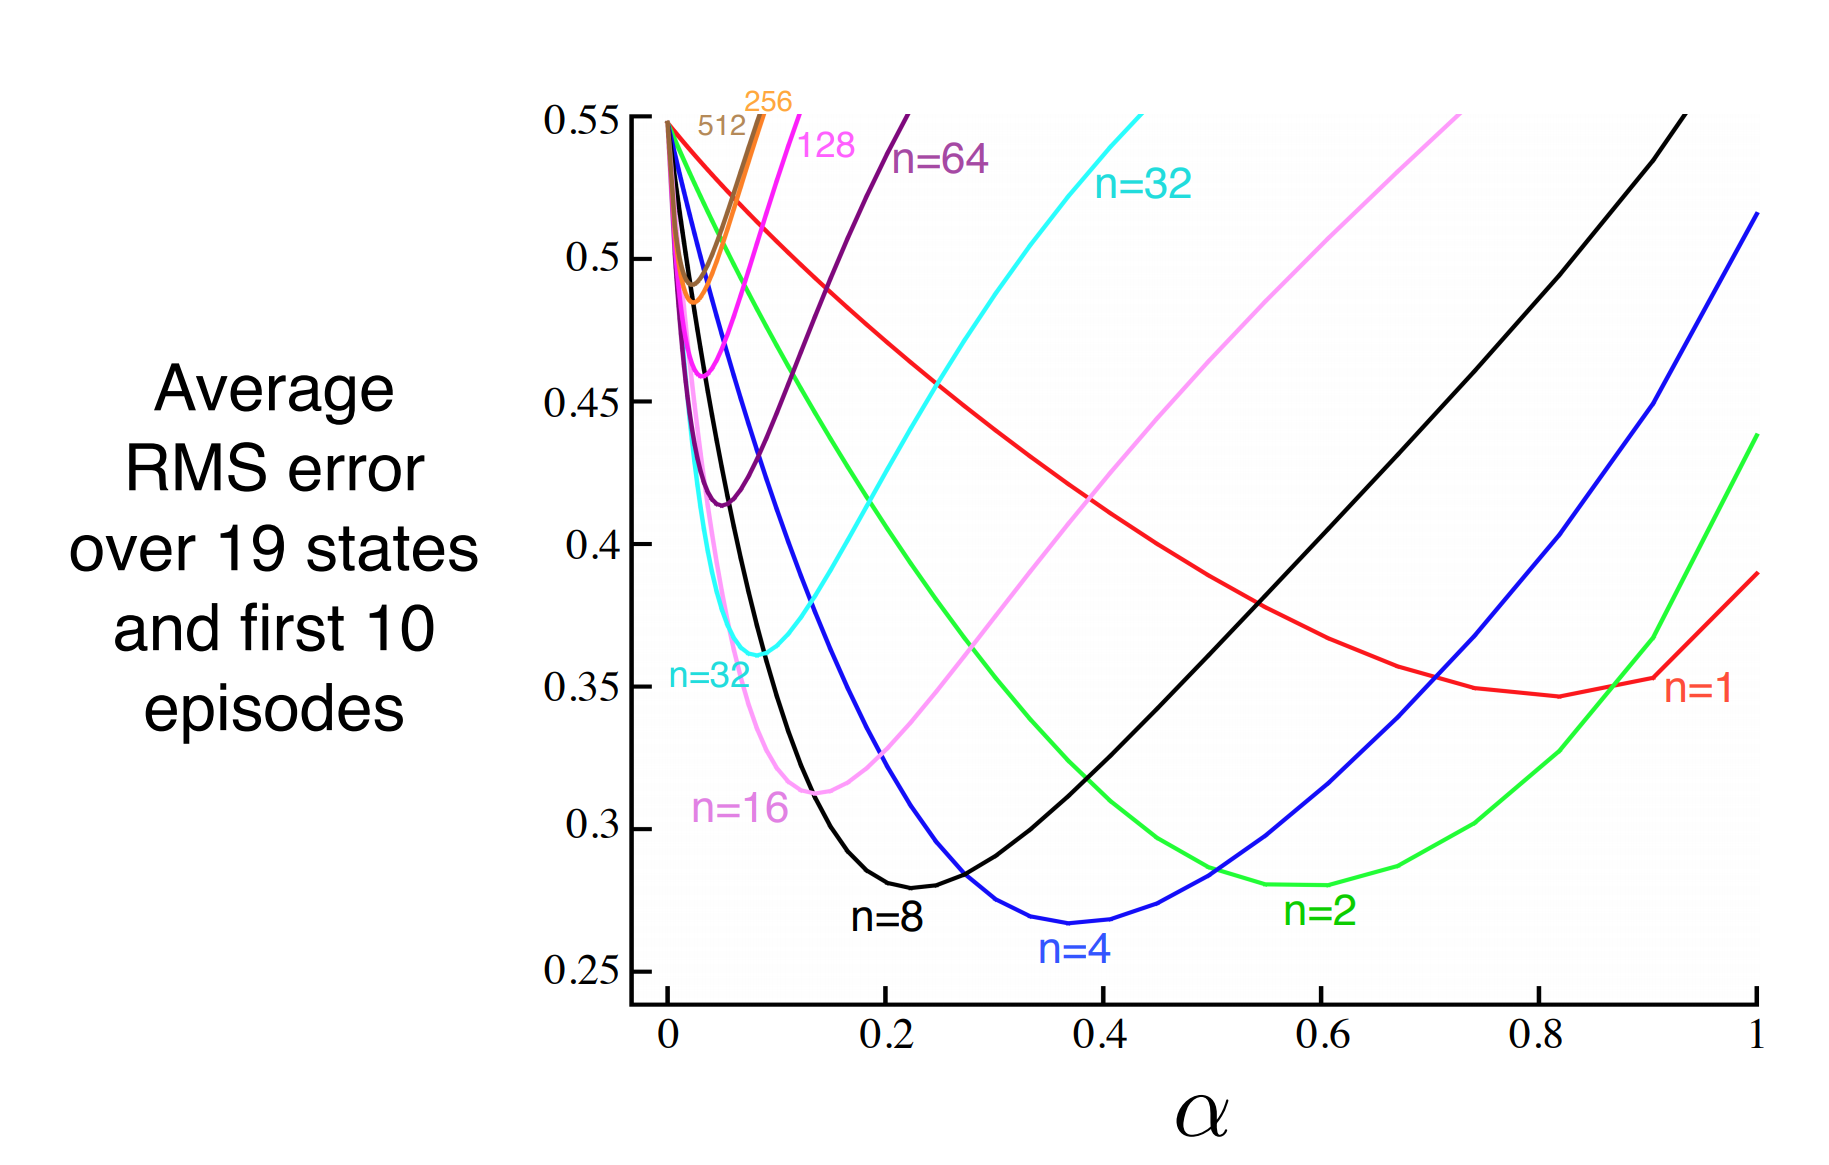
\includegraphics[scale=0.12]{bias_variance.png}
    \captionsetup{width=.7\textwidth}
    \caption{\textbf{RMS error on a toy example given different $n$-step updates}. A 4-step update is seen to achieve the best performance. The plot and more information about the toy example can be found on page 145 in \cite{sutton_barto_2018}}.
    \label{fig:bias-variance}
\end{figure}

\subsubsection{Q-Learning}

One issue that remains with the aforementioned methods is that they are \textit{on-policy}. This means that in order to update the value function of a policy one has to use transition experiences following the policy. This means that if the policy is changed, a new set of transition experiences are required to keep training. This means that an agent must be given direct access to the environment to learn new policies and decreases the amount of data that can be used for training. 

\cite{watkins_dayan_1992} marked a large step forward in reinforcement learning through the development of an off-policy temporal difference method. The method is based on the action-value function (\ref{eq:act_value_function}) and is called Q-learning.

\begin{equation}
    \label{eq:td_q_learning}
    Q(S_t, A_t) = Q(S_t, A_t) + \alpha\big[R_{t+1} + \gamma \max_a Q(S_{t+1}, a) - Q(S_t, A_t)]
\end{equation}

Note that this equation is completely independent of the policy followed when generating the experience. This means in contrast to an on-policy method, Q-learning can be trained on transition experiences from any policy regardless of what the Q-learning policy is.

\subsection{Exploration vs Exploitation}

Given the correct action-value function, the optimal policy will be to pick the action with the highest Q-value.

\begin{equation}
    \label{eq:greedy}
    A_t = \argmax_a Q_t(a)
\end{equation}

The policy defined in equation \ref{eq:greedy} is known as a greedy policy and following this policy is called \textit{exploiting} the policy. Note that in contrast to a greedy method in computer science, this greedy policy does take into account future events through the reward propagated through the bellman equation.

The issue with this policy is that one does not have the correct action-value function. It will always pick what is the estimated best action without picking new actions to test if it will lead to an even better reward. In other words, the greedy policy will never \textit{explore} the environment and therefore might miss a better policy.

A balance is needed between exploiting the policy to maximize reward and exploring to find a better policy. A simple solution to this problem is the $\varepsilon$-greedy policy 

\begin{equation}
    A_t = \begin{cases}
        \argmax_a Q_t(a) &\quad \text{with probability} \quad 1-\varepsilon \\
        a \sim \text{Uniform} (\mathbb{A})  &\quad \text{with probability} \quad \varepsilon.
    \end{cases}
\end{equation}

where $0 < \varepsilon < 1$ and $\mathbb{A}$ is the set of all legal actions.
Asymptotically this policy is guaranteed to visit every state an infinite amount of times. This generally works quite well in practice but can be inefficient for complex environments. \citep[p.~27-28]{sutton_barto_2018}

\section{Deep Q-Learning}

\subsection{Function Approximation}

The reinforcement methods discussed in the previous section are called tabular methods as they consist of saving a value for each state or an action-value for each state action pair. These methods have two major shortcomings \cite[p.~195-196]{sutton_barto_2018}. Firstly when either the action or state space becomes sufficiently large, this representation becomes impractical due to memory constraints. For example, the game of chess has a state space of magnitude $10^{43}$\citep{shannon_1950} so creating a dictionary mapping from state to value is impossible with current technology. 

The second issue is generalization. The tabular methods discussed require many visits to each state and action of interest to have an accurate action-value estimate. Given an unvisited state there will be no good estimate of the action-values for the policy to be based upon. The tabular method does not generalize to new or even rarely visited states.

To illustrate this consider the environment of buying and selling stock while maximizing profit. Take for example the Apple stock prices and define the state as the differenced opening prices rounded to the nearest cent. Figure \ref{fig:stock_diff}A shows that small changes in price are most common. Therefore one expects good value approximations at these price changes. However for larger changes in prices there is less or no data. If in evaluation the environment results in a large price drop that hasn't been seen before the tabular methods will have no action-value estimates leading to no policy to follow. This is not only a problem for large price changes. Zooming in on the price data as in figure \ref{fig:stock_diff}B shows that there are certain low price changes that have limited data. For these the same problem will occur.

\begin{figure}[H] %this figure will be at the right
    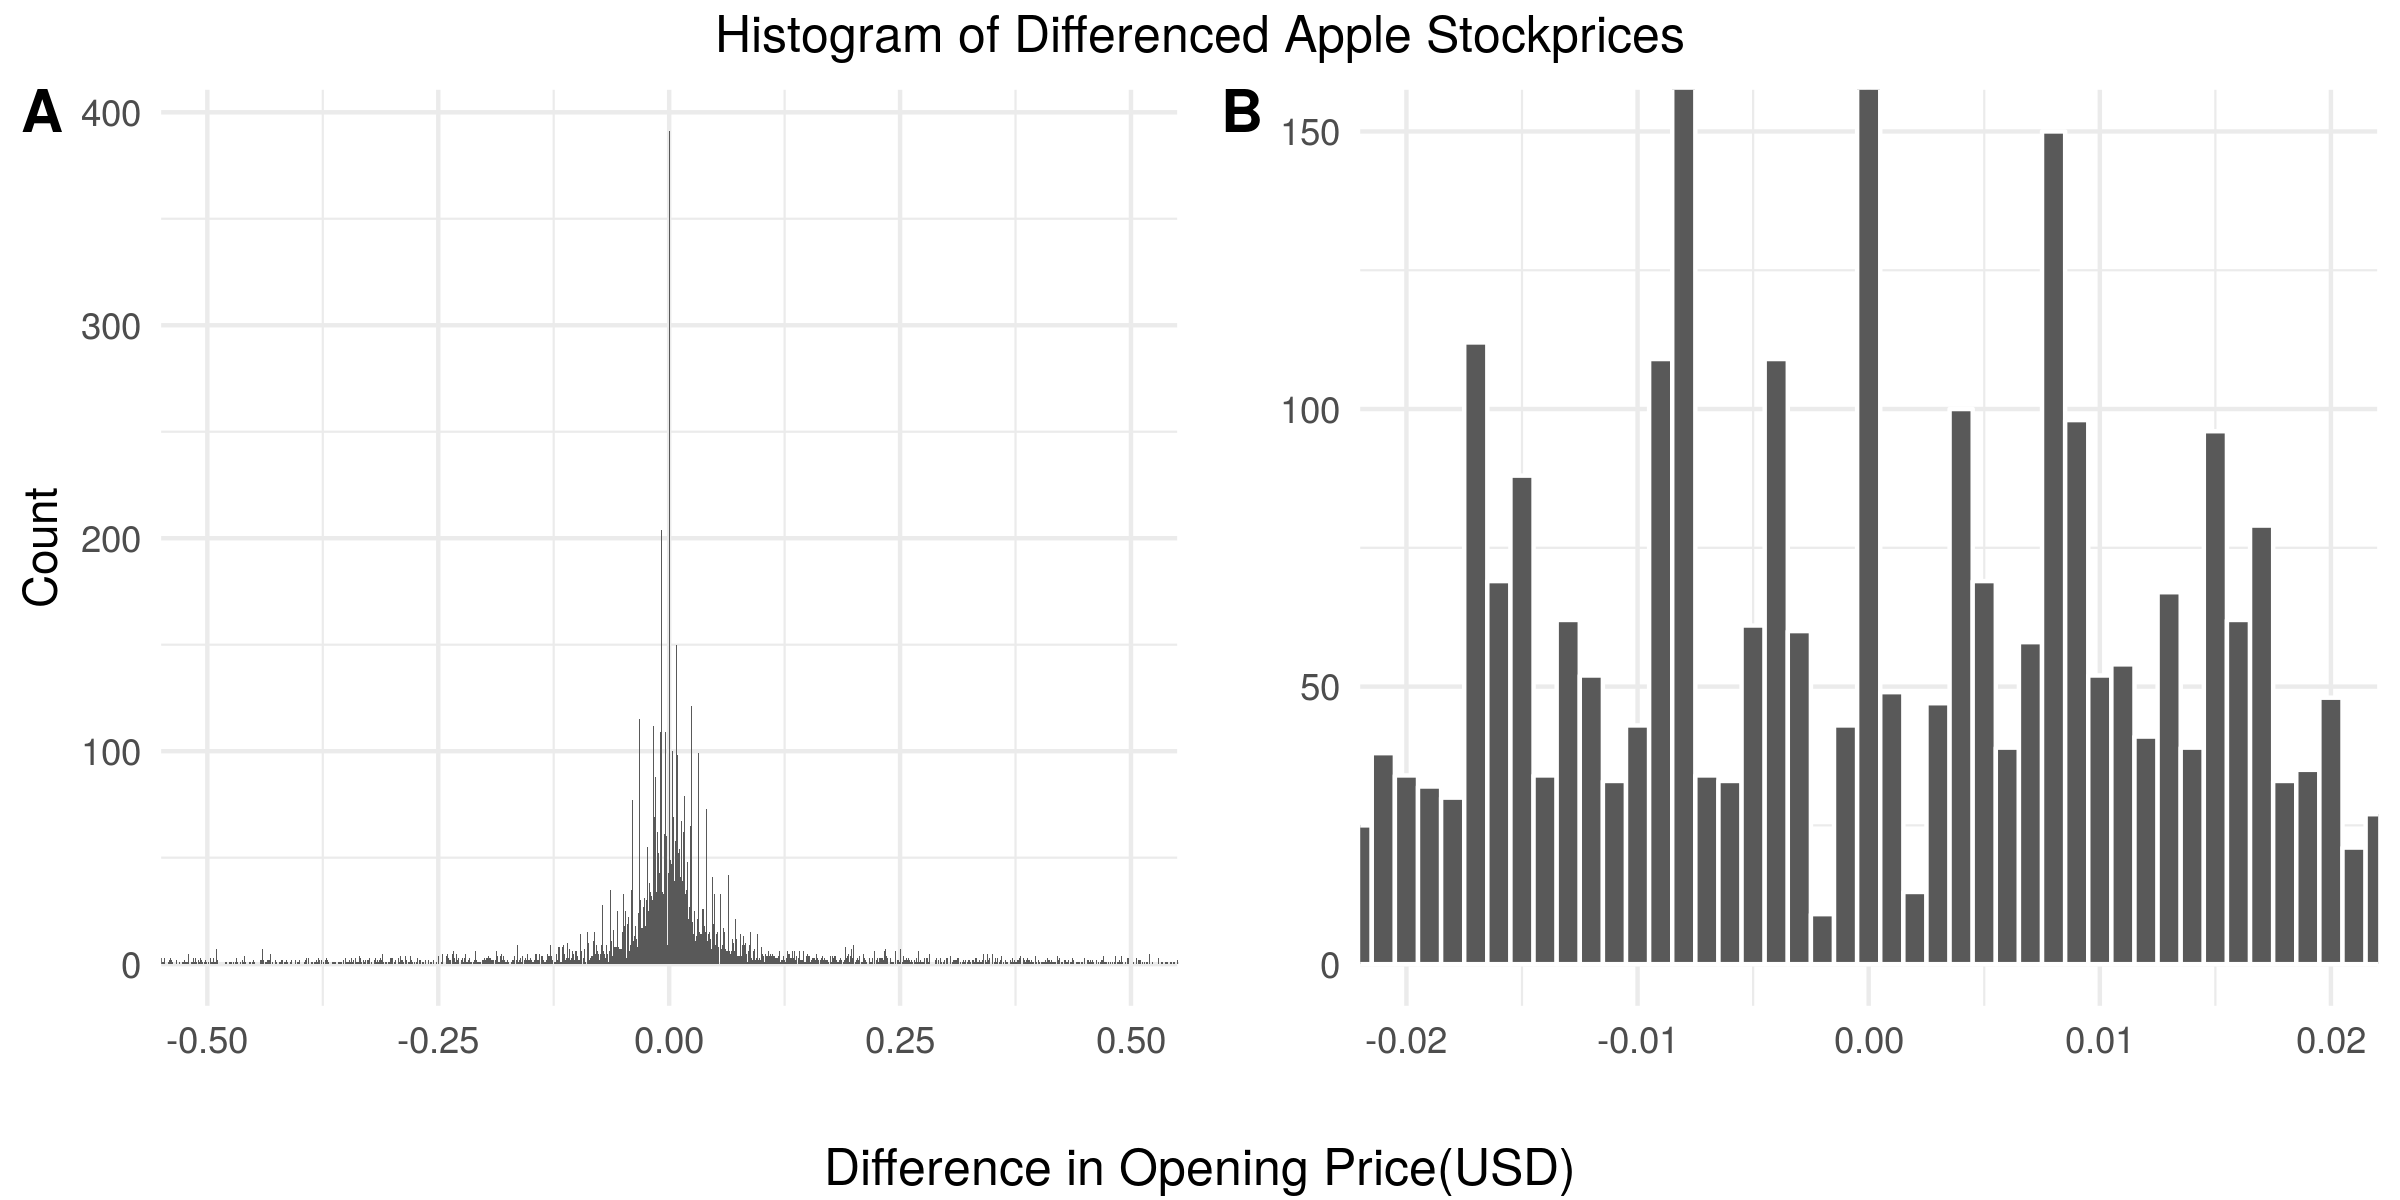
\includegraphics[width=\textwidth]{stock_diff.png}
    \caption{\textbf{Differenced Apple Stock Opening Prices}}
    \label{fig:stock_diff}
\end{figure}

Ideally the value estimate the method should be able to generalize to states with limited experiences or completely unseen states. In the stock price example the value and policy at similar prices should give information about how the agent should act given an unseen price. 

The approach to solving this is using function approximation. When estimating the value or action-value function one is trying to estimate a continuous value given a set of input values. This is a regression problem. So instead of using a table to map states to values one can use regression methods to do the same. 

Since the value function is dependent on the policy and the policy is changing during training, the target is non-stationary. It is therefore important that the regression method chosen must be able to deal with non-stationary targets.\cite[p.~198-199]{sutton_barto_2018}

It is important to note that using function approximation means that the convergence guarantees discussed earlier no longer hold. Some function approximation methods are still guaranteed to converge to a policy, albeit not necessarily the optimal policy while others are unstable and require special tweaks to reliably converge to a policy. Specifically off-policy methods with function approximation will sometimes diverge but in practice they tend to converge\citep[p~.258]{sutton_barto_2018}.

\subsection{Linear function approximation with Q-learning}

In linear Q-learning the goal is to create a regression model that maps the state and action to a Q-value, $Q(s,a)$. Let $x_t$ denote the state and action at timestep $t$. $X$ then denotes the design matrix containing these features and $Q$ the vector of corresponding Q-values. The regression model for a single action can then be defined as

\begin{equation}
    \label{eq:regression}
	Q(X) = X\beta + \varepsilon \quad \text{where} \quad \varepsilon \sim N(0,\sigma^2)
\end{equation}

with the response value defined as 

\begin{equation}
    \label{eq:q_target}
	Q(s,a) = r_t + \gamma\argmax_{a'}Q(s',a').
\end{equation}

The ordinary least squares solution to the $\beta$ coefficients can then be found using the normal equation \citep[p~.105-107]{fahrmeir_2013} which in matrix form is

\begin{equation*}
	\beta = [X^TX]^{-1}X^TQ.
\end{equation*}

However this method is under the assumption that the target distribution is stationary and has to be trained on the entire dataset when given new data. This makes it ill-suited for reinforcement learning where one is constantly receiving new data from a non-stationary distribution. 

Instead the common approach is to apply stochastic gradient descent over the parameters \citep[p~.201-203]. With a monte carlo target this gives the equation 

\begin{equation*}
    \beta = \beta + \alpha \big[G_t - Q(s,a|\beta)]\nabla_\beta Q(s,a|\beta).
\end{equation*}

The same equation for the temporal difference target gives 

\begin{equation*}
    \beta = \beta + \alpha \big[ r_t + \gamma\argmax_{a'}Q(s',a'|\beta) - Q(s,a|\beta)]\nabla_\beta Q(s,a|\beta)
\end{equation*}

Note that in the temporal difference case the target is dependent on the coefficients and therefore does not fulfill all the criteria for stochastic gradient descent. This results in losing the guarantee that the method converges to a local optimum. However empirically in the case of linear models it tends to reliably converge.

Given this model the agent can take an action by acting greedily over the models $Q(s,a)$ values in a given state. Since this is purely an exploitation strategy, it is often coupled with the $\varepsilon$-greedy policy.

\subsection{Nonlinear function approximation}

Action-value functions can be complicated functions so it can be desirable to have a nonlinear function approximator.

\subsubsection{Fully Connected Neural Networks}

One popular class of nonlinear models are neural networks. This class covers a large variety of models. The simplest and perhaps most used model is the fully connected(F neural network(NN). A fully connected NN consists of sets of neurons, called layers, where each neuron receives an input from every neuron in the previous layer.

A neuron is simply either a regression or classification model where the output is passed through a function named the activation function. This function is usually non-linear to allow the NN to model non-linear functions. Mathematically a neuron is expressed as 

\begin{equation}
    Z = \sigma(W^TX)
\end{equation}

where $X$ is the vector of inputs from the previous layer, $W$ are the coefficients of the regression or classification and $\sigma$ is the activation function.

The coefficients of regression/classification are called weights. These are the unknown parameters in the model that must be estimated. To do this a loss function must be defined. There any many choices of loss function. Two common choices are mean square error(MSE) for regression problems and cross-entropy for classification problems. 

MSE is defined as 

\begin{equation}
 L(\bm{\theta}) = (y - \hat{y}(\bm{\theta}))^2
\end{equation}

while cross-entropy is

\begin{equation}
 L(\bm{\theta}) = -y \log \hat{y}(\bm{\theta}).
\end{equation}

The weights that minimize these losses around found through gradient descent. The weights in layer $k$ are updated by the formula

\begin{equation}
 w_k = w_k - \gamma \frac{\partial{L}}{\partial{w_k}}
\end{equation}

where $\gamma$ is known as the learning rate and controls the step size of the optimization.

The implementation of this can be simplified through the use of the back propagation equations. Using chain differentiation with the MSE loss function it can be shown that 

\begin{equation}
    \begin{split}
        &\frac{\partial{L}}{\partial{w_K}} = \delta_K z_K \\
        &\frac{\delta{L}}{\delta{w_k}} = \delta_k z_{k-1}\\
        \text{where} \quad &\delta_K = \nabla L(w_K)\circ\sigma'(w_K z_{K-1})\\%-2(y - z_K)\sigma'(w_K z_{K-1}) \\
        & \delta_k = \sigma'(w_k z_{k-1}) \sum_{i=1}^{S_k}\big(w_{k+1}\delta_{k+1}\big)
    \end{split}
    \label{eq:backprop}
\end{equation}

where $S$ is the size of the layer, $K$ denotes the final layer and $\sigma$' is the differentiated activation function. The above allows the gradients to be calculated based on the gradient calculation for next layer. To train the network the prediction is calculated by a forward pass through the network and then the weights are updated by calculating the above for each layer in backward order. \citep[p.~ 392-396]{hastie_2009}

\subsubsection{Q-learning with Neural Networks}

To use neural networks as a nonlinear function approximator in RL the only step left is defining the loss in the RL setting. Consider the case of trying to minimize the mean square error of the action-value estimate

\begin{equation}
    L_i(\theta_i) = \mathbb{E}_{s,a}\Big[\big(y_i - Q(s,a;\theta_i\big)^2\Big]
\end{equation}

where $\theta$ are the parameters of the model being used. As this project focuses on temporal difference methods the target is set to the same as in Q-learning (equation \ref{eq:td_q_learning}).

\begin{equation}
    y_i = \mathbb{E}_{s'}\big[r+\gamma \max_{a'} Q(s', a'; \theta_{i-1})|s,a\big]
    \label{eq:Q_target}
\end{equation}

The loss function can then be differentiated with respect to the model parameters resulting in 

\begin{equation}
    \label{eq:RL_gradient_descent}
    \nabla_{\theta_i}L_i(\theta_i) = \mathbb{E}_{s,a; s'}\Bigg[\Bigg(r+\gamma\max_{a'}\bigg(Q(s',a';\theta_i)\bigg)-Q(s,a;\theta_i)\Bigg)\nabla_{\theta_i}Q(s,a;\theta_i)\Bigg]
\end{equation}

which can then replace $\nabla L(w_K)$ in equation \ref{eq:backprop}.

\subsubsection{Convolutional Neural Networks}

Certain methods in this thesis will also use convolutional neural networks(CNN) in combination with fully connected NNs. This is not vital to the understanding of the work done in this thesis so only a brief intuition of CNNs will be provided. The following is summarized from chapter 9 in \cite{goodfellow_2013}.

Images are high dimensional so running fully connected NN that maps from every input to some final output requires a lot of parameters and is computationally heavy. In addition many of these parameters are wasted the same feature in different parts of the image should lead to similar results. In a fully connected NN this feature would have to be relearned  for each location it can appear in an image. In addition if a feature ends up in a new position that the NN has not be trained on the method will fail.

CNNs are a different NN structure designed towards use cases such as images.  A convolution operator is essentially a weighted sum of some input. In an image the weighted sum is over a local neighborhood based on the inputs position. CNNs learn a small set of weights and repeatedly takes the convolution between these a subset of the input across the entire input. Usually a CNN consists of many sets of these weights which learn different features. The result of this is that a CNN can recognize features regardless of their placement, known as translation invariant, and so does not need to relearn the same encodings. This means a CNN can recognize features with far less features and better generalizability than a regular NN.

\subsubsection{The Deadly Triad}

There is an issue that arises with function approximation, which is known as the deadly triad. When combining function approximation, bootstrapping and off-policy training one often finds that the estimate becomes unstable and can diverge. This is especially a problem with nonlinear function approximators like neural networks \citep{mnih_2013}. Dropping one of these factors essentially negates this problem, however using all of these is desirable due to their contribution to an increase in performance. \cite[p.~264-265]{sutton_barto_2018}.

\subsection{Deep Q Networks}

The recent rise in interest in NN led to research in using these as a nonlinear approximator for Q-learning. In \cite{mnih_2013} a method called the Deep Q Network (DQN) was introduced achieving state of the art results on a select few Atari games. They used a multilayer NN Q-value function approximator that takes in a state $S$ as input and outputs a Q-value per action. For exploration they follow a $\varepsilon$-greedy policy starting with $\varepsilon=1$ that decreases towards to $\varepsilon=0$ as training progresses.

Due to the deadly triad issues, some modifications had to be made to Q-learning to handle the divergence issues. To deal with this \cite{mnih_2013} reintroduced a concept called \textit{experience replay}, originally introduced in \cite{lin_1993}. Instead of training the network after every step taken, experiences are saved as the tuple $e_t=(s_t, a_t,r_t, s_{t+1})$ creating a data set of experiences $\mathcal{D} = e_1,...,e_n$. The neural network can then be trained using samples drawn randomly from $\mathcal{D}$. In practice this is done every few steps taken by the agent.

\cite{mnih_2015} further increased stability by using two neural networks instead of one. The second neural network, called the target network, is used to calculate the target $Q$ value, the $Q(S_{t+1}, a)$ term in equation \ref{eq:td_q_learning}. The weights of the target network are copied from the original network, called the online network, after a large number of steps. This creates a more stable optimization target. 

In addition, instead of using the MSE \cite{mnih_2015} suggests clipping the gradient of the loss function to be between -1 and 1 as they observed it lead to more stable learning. Since one only uses the derivative of the loss function in this application this is the equivalent of using the Huber loss function \ref{eq:huber_loss}

\begin{equation}
    \label{eq:huber_loss}
    L(y, \hat{y}) = \begin{cases}
        (y-\hat{y})^2 \quad \text{for } |y-\hat{y}| \le 1 \\
        2|y-\hat{y}| - 1\quad \text{otherwise}.
    \end{cases}
\end{equation}

as it is defined in \citep[p.~349]{hastie_2009}.

The DQN version from \cite{mnih_2015} achieved new state of the art results on a much larger set of Atari games and has become a standard baseline for RL methods.

\subsection{Further developments on DQN}

Many additional tweaks to DQN have been introduced since \cite{mnih_2015}. Some of the more promising changes were combined and tested in \cite{hessel_2017}. To decrease the experiment run-time this project implements one of the changes mentioned in \cite{hessel_2017}, namely the double DQN.  This change is not fundamental to this project so it will only be briefly discussed.

\cite{hasselt_2010} showed that tabular Q-learning can have large positive bias in certain environments. This was due to an overestimation as a result of the max operator. To fix this they suggested creating two separate action-value functions and replacing the Q-learning update with 

\begin{equation}
    \begin{split}
    Q_2(s,a) &= Q_2(s,a) + \alpha\bigg(r + \gamma Q_1\big(s', \argmax_{a'}[Q_2(s',a')]\big) - Q_2(s,a)\bigg) \\
    Q_1(s,a) &= Q_1(s,a) + \alpha\bigg(r + \gamma Q_2\big(s', \argmax_{a'}[Q_1(s',a')]\big) - Q_1(s,a)\bigg).
    \end{split}
\end{equation}

During training one randomly picks one update to run every step. The underlying idea is that one decouples the targets action selection from its value estimation which results in a less biased estimator. In \cite{hasselt_2015} this is extended to the DQN by simply using the target Q-network $Q'$ as the second action-value function. The target Q-value was then calculated by

\begin{equation}
    R_t + \gamma Q'(S_{t+1}, \argmax_{a'}Q(S_{t+1}, a')).
\end{equation}

This is not equivalent to a complete decoupling of two action-value functions but empirically this reduced the bias and thus improved performance. 

\subsection{Limits of DQN}

Despite the human-level performance of DQN methods in many Atari games \citep{mnih_2015} there are still some games DQN fails to complete successfully. These games have proved to be difficult to despite developments in RL \citep{mnih_2016, schulman_2017, hessel_2017}. One game of particular interest in the RL research community is Montezuma's revenge. This environment has sparse rewards with many policies leading to a quick loss. In this case modern RL methods fail to explore efficiently to reach any successful policy.

\section{Exploration through uncertainty}

Despite the guarantee that $\varepsilon$-greedy will asymptotically explore all states this might not always be computationally feasible. Even if it is computationally feasible, the sample efficiency of RL is known to be quite bad. One of the most sample efficient methods within Atari games is \cite{hessel_2017} but this still required 20 million frames per game to achieve its results. Since $\varepsilon$-greedy uses no information about the environment or agent a focus of research has been to perform more informed exploration. 

\subsection{Uncertainty in Reinforcement Learning}

Knowing the variance of the Q-value estimate gives an insight into how certain the model is about the Q-value. This can be used to pick actions that are estimated to be sub-optimal but could have higher (or lower) Q-values due to uncertainty. However calculating this variance isn't as simple as a regular regression setting.

\subsubsection{Propagation of Uncertainty}

To understand the challenge of variance in RL, first consider a naive attempt at incorporating variance in action selection. Assuming that the variance of an estimate is proportional to the inverse visit count to a state one can define the policy

\begin{equation}
    A_t = \argmax_a \Bigg[Q_t(a) + c\sqrt\frac{ln(t)}{N_t(a)}\Bigg].
    \label{eq:ucb}
\end{equation}

This can be viewed as setting the Q-value to be the upper confidence bound of the Q-value \citep{strehl_2008}\citep[p.~35-36]{sutton_barto_2018}.

This assumes that future returns come from a stationary distribution. In reality this assumption is often wrong. As the agent's policy changes, the future returns change, which implies an non-stationary distribution. This means that the variance of a Q-value is dependent on the variance of Q-value estimate along with the variance of future Q-values due to the uncertainty in the agent's policy. Therefore, in the same way Q-values must be propagated from future Q-values, the variance of the Q-value must be propagated from the variance of future Q-values. \citep{moerland_2017}

To illustrate the issue, consider the chain example from \cite{osband_2016}. Consider N states connected in a chain as in figure \ref{fig:chain}. The agent starts in $S_1$ and has two actions; move left or right. Transitioning to $S_1$ gives a reward sampled from $\mathcal{N}(0,1)$, $S_N$ gives a reward from $\mathcal{N}(1,1)$ and the rest of the states result in no reward.


\begin{figure}[H]
    \centering
    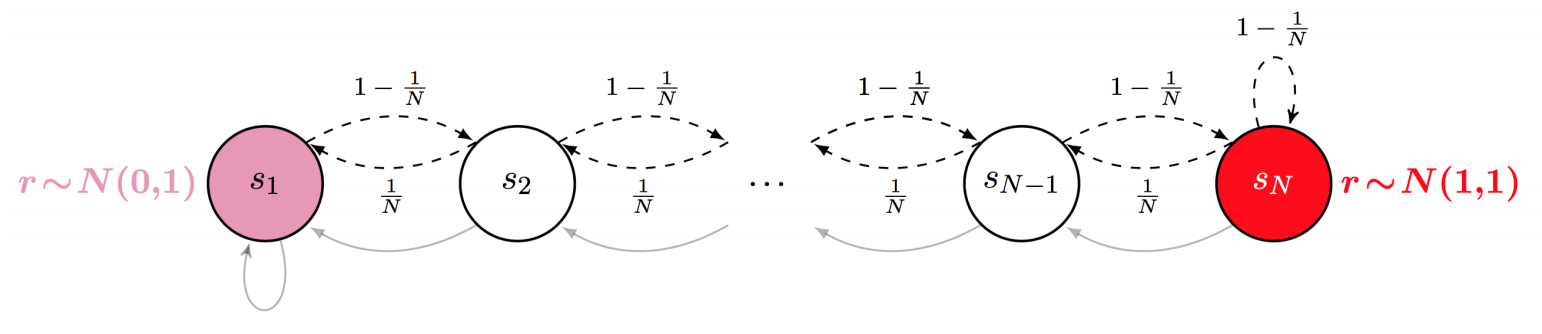
\includegraphics[width=\textwidth, keepaspectratio]{chain.png}
    \caption{\textbf{Chain environment}. The figure is taken from \cite{osband_2016}}
    \label{fig:chain}
\end{figure}

The optimal policy is to always move right. However an agent following the policy in equation \ref{eq:ucb} will quickly end up underestimating the value of states too the right as multiple visits to $S_2$ would lead to a low exploration bonus despite the fact that states further to the right have not been properly explored. If this occurs before the agent reaches $S_N$ it will never find the higher reward to the right and end up with a suboptimal policy.

\subsubsection{Optimism in the Face of Uncertainty}

One method to propagate the uncertainty from future value estimates is to include the exploration bonus in the Bellman equation. This is done with the value function in \cite{strehl_2008}:

\begin{equation}
    \max_a \mathbb{E}\Big[R_t+\gamma V(S_{t+1})+\beta N(S,a)^{-\frac{1}{2}}\Big].
\end{equation}

If one considers the uncertainty around the value to be an interval of statistically plausible values, this method optimizes the Bellman equation over the highest statistically plausible value. This has given the method the name optimism in the face of uncertainty(OFU). This method is only applicable to tabular environments and fails for large state spaces where visit counts tend to be low.

\cite{bellemare_2016} generalized this equation away from relying directly on visit counts by estimating a visit count from a linear approximation model. This achieved state of the art results in multiple environments when published. However, an issue with this method is that it changes the loss function which no longer directly optimizes the Bellman equation. This can lead to inefficient exploration at times or sub-optimal behavior \citep{moerland_2017}. In addition the method used both temporal difference and monte carlo updates, which the paper itself states lead to major improvements.

\subsection{Posterior sampling for reinforcement learning}

A second paradigm in uncertainty based exploration is posterior sampling for reinforcement learning (PSRL). This method builds on a bayesian view of reinforcement learning. Considering the task of maximizing reward from an MDP. Bayesian reinforcement learning treats the unknown MDP as a random variable. To do this one considers the expected one-step reward $\hat{R}^*(s,a)$ and transition probabilities $P^*(s,a)$ to be random variables. Denoting a sample from these distributions as $r^*$ and $p^*$ one can create a posterior sample of the action-value $Q^*$ conditioned on the history of transitions by using the following equation. 

\begin{equation}
 \label{eq:bayesian_bellman}
 Q^*(s_t,a_t) = \hat{R}^*(s,a) + \sum_{s_{t+1}, a_{t+1}}P^*(s_{t+1}|s_t,a_t)\max_{a'}Q^*(s_{t+1}, a_{t+1})
\end{equation}

The PSRL method then defines the policy by greedily picking the best action over a posterior sample of each available action-value. This is known as Thompson sampling. \citep{strens_2000}\citep{osband_2016}

\begin{equation}
a_t = \argmax_{a\in\mathcal{A}} Q^*(s_t,a)
\end{equation}

To grasp the intuition to why the above leads to exploration consider an environment with only two actions. Assume that the action-value posterior is gaussian and that there are two actions to choose from as shown in figure \ref{fig:posterior-qvalues}.
 
\begin{figure}[H]
\centering
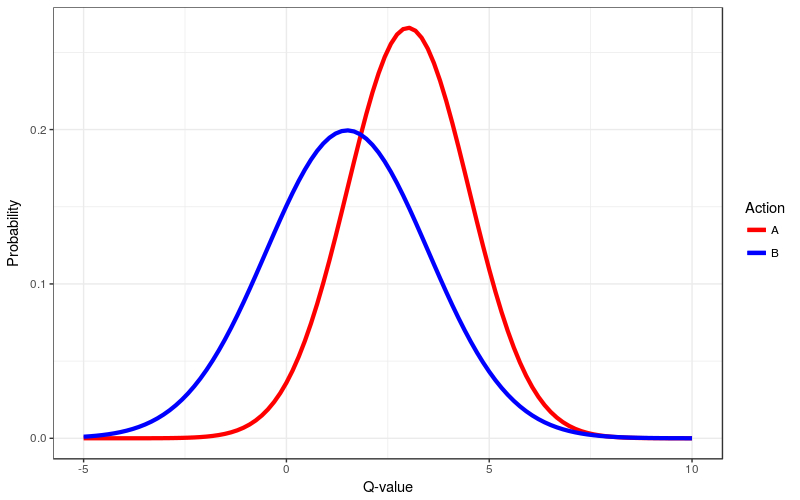
\includegraphics[width=0.5\textwidth, keepaspectratio]{posterior_actions.png}
\captionsetup{width=.7\linewidth}
\caption{\textbf{Posterior distribution of action-values:} Despite action A having a higher expected value, the posteriors indicate that action B could potentially be the best action.}
\label{fig:posterior-qvalues}
\end{figure}


Figure \ref{fig:posterior-qvalues} shows that the expected Q-value of action A is higher than B. However, the posterior distribution of Q-values can be viewed as the distribution of plausible values for Q \citep{osband_2016}. The overlap between the two distributions indicates that there is a certain probability that action B is actually better than action A. By sampling these posteriors when chosing action one gives a probability of choosing action B over action A that is related to the amount of overlap between these distributions.

\cite{osband_2016} shows that the sample-efficiency scales better with respect to the number of states and actions for posterior sampling than optimism in the face of uncertainty. However, the challenge remains in finding a good posterior that is not so computationally heavy that it cancels out the sample-efficiency.

\section{Recent Research within Deep PSRL}

Computationally tractable methods for bayesian inference in neural networks is especially challenging. Despite this there are multiple recent papers within that have been released the past year that are able to generalize PSRL to deep RL. Most of these use some form of approximation to simplify sampling from the posterior Q-value. A summary of three recent deep PSRL papers that are well cited and have helped form this thesis are provided.

\subsection{Randomized Prior Functions for Deep Reinforcement Learning}

\cite{osband_2018} finds an approximation to the posterior Q-value distribution through a mixture of statistical bootstrapping and ensemble methods. First the method assumes the posterior to be a gaussian distribution. It then presents the following, slightly summarized, lemma:

\textit{Let $f_\theta (x) = x^T\theta$, $\tilde{y}_i\sim N(y_i,\sigma^2)$ and $\tilde{\theta} \sim N(\bar{\theta}, \lambda I)$. Then the following optimization problem generates a sample $\theta | \mathcal{D}$}

\begin{equation}
    \tilde{\theta} + \argmin_\theta \sum_{i=1}^n\|\tilde{y}_i-(f_{\tilde{\theta}} + f_\theta)(x_i)\|_2^2 + \frac{\sigma^2}{\lambda}\|\theta\|_2^2.
\end{equation}

Breaking down this statement the method starts by sampling coefficients $\tilde{\theta}$ from the prior to create a prior function $f_{\tilde{\theta}}$. Then it fits an additive model $f_\theta(x)$ with a regularization term $\frac{\sigma^2}{\lambda}\|\theta\|_2^2$ to a noisy version of the dataset $\tilde{y} \sim N(y, \sigma^2)$. The resulting outputs from $(f_{\tilde{\theta}}-f_{\theta})(x_i)$ will be a single sample from the posterior. 

This means that in order to model the posterior based on $n$ samples one needs $n$ models. Though it can be computationally heavy to create many models it is also noted that these models can be trained in parallel, meaning this method is scalable given the right computational resources.

To generalize to neural networks the method approximates further by replacing the prior model with a fixed randomly initialized neural network $p$ multiplied by a hyperparameter $\beta$ that regulates the magnitude of the prior. Instead of applying noise to the data a new dataset is created by statistically bootstraping the original dataset. A separate DQN is then trained on the bootstraped data and the addition of the fixed prior network. The resulting Q-value is then 

\begin{equation}
    Q(s,a) = f_\theta(s,a) + \beta p(s,a)
\end{equation}

The paper then shows that on hard exploration toy examples such as a variant on the chain environment(figure \ref{fig:chain}) the method far outperforms an $\varepsilon$-greedy exploration policy. In addition the method manages to escape the first room in Montezuma's Revenge, receiving an average score of approximately 2500. However the paper also notes that this performance is sensitive to adjustments to the prior scale $\beta$.

\subsection{The Uncertainty Bellman Equation and Exploration}

The specialization project that preceded this work was an investigation into \cite{donoghue_2017}. They introduce an upper-bound on the variance of the Q-value based on the Bellman equation

\begin{equation}
    \var Q(s,a) \le \nu(s,a) + \sum_{s',a'}\mathbb{E}\big[P(s'|s,a)\big]\var Q(s',a')
\end{equation}

where $\nu$ is given by

\begin{equation}
    \nu(s,a) = \var \mu_r(s,a) + Q_{max}^2 \sum_{s'} \var \frac{P(s'|s,a)}{\mathbb{E}\big[P(s'|s,a)\big]}.
\end{equation}

$\nu$ is called the local uncertainty since it only depends on the current state-action pair and not the variance of future action-state pairs.

By assuming the variance is the upper-bound value \cite{donoghue_2017} one gets a bellman style equation

\begin{equation}
    u(s,a) = \nu(s,a) + \sum_{s',a'}\mathbb{E}\big[P(s'|s,a)\big]\var Q(s',a')
\end{equation}

which, when based on experiences rather than model dynamics gives

\begin{equation}
    u(s,a) = \nu(s,a) + \gamma^2 u(s',a').
\end{equation}

Given a method to calculate $\nu$ this allows one to learn the $u(s,a)$ values using the same methods used to learn $Q(s,a)$.

It is then assumed that there are enough experiences to use the central bayesian limit theorem. This implies that the posterior distribution of the $Q^*$-value is approximately distributed by a normal distribution\citep[p.~224]{berger_1985}. As such, given a $\mathbb{E}[Q]$ value from any regular Q-learning method and a variance calculated from the UBE one can sample a posterior $Q$-value from the distribution $N\bigg(\mathbb{E}\big[Q(s,a)\big], u(s,a)\bigg)$.

The issue that remains is how to calculate the local uncertainty $\nu$. \cite{donoghue_2017} argues that $\nu$ can be approximated by action-value models variance. Given a target $y_i$ with i.i.d. variance it can be shown that for a linear regression with weights $w_a$, a new input $\phi(s)$ and design matrix $\bm{\Phi}$ the model variance is $\phi(s)^T\bm{\Phi}^T\bm{\Phi}\phi(s)$. The local uncertainty is the estimated by

\begin{equation}
    \nu(s,a) = \beta^2\phi(s)^T\bm{\Phi}^T\bm{\Phi}\phi(s)
\end{equation}

where $\beta$ is a hyperparameter that controls the scale of the local variance and represents the actual variance of the target.

By ignoring the uncertainty in the neural network encoding the same logic can be applied to the final layer in a DQN. The final deep RL implementation creates a DQN with two heads. Head one is trained as a regular DQN and outputs Q-values. Head 2 is trained using the UBE with local uncertainties calculated from the final linear layer from head 1.

Actions are then chosen by sampling the normal distribution with the mean estimate from head 1 and variance estimate from head 2. With this method \cite{donoghue_2017} managed state of the art results on Montezuma's Revenge when published. In addition it allowed, under heavy assumptions that are broken, sampling from an approximated posterior using a DQN model that only took 10\% more computation to run, rather than the $n$ times heavier computation for ensemble methods.

\subsection{Efficient Exploration through Bayesian Deep Q-Networks}

\cite{azziz_2018} will be discussed in detail in chapter \ref{ch:linear} so only a brief overview of the paper is provided here. The paper consists of two major results of which the first is relevant to this thesis. This part introduces a deep RL PSRL method they denote the Bayesian Deep Q-Network (BDQN). 

The BDQN assumes a gaussian prior and posterior distribution. It then replaces the final linear layer in the DQN with a bayesian linear regression. This allows a DQN that can sample Q-values from a posterior, albeit one that ignores uncertainty in the network encoding. Note that this method does not explicitly propagate uncertainty and chapter \ref{ch:linear} will argue that the method has no uncertainty propagation. In addition, as in \cite{donoghue_2017} and \cite{osband_2018} the variance scale is set as a hyperparameter.

Since this thesis will be heavily discussing the BDQN it is also worth noting that \cite{azziz_2018} has not been accepted to any conference at the time of writing. Despite this the paper is well known in the RL field with over 30 citations and is often brought up in new PSRL papers. An open review for ICLR 2019 shows that the concerns about this paper revolve mainly around the second part of the paper, a theoretical proof of performance, not the BDQN\citep{openreview_bdqn}.

\subsection{Dropout}

On a short note, if the reader is well-versed in neural networks one might wonder why none of these paper use dropout to estimate the posterior. In this case it is recommended to view the discussion in \cite{osband_2018} about the shortcomings of dropout in RL. In addition \cite{azziz_2018} empirically shows that dropout does not perform well in the RL setting.

\cleardoublepage